\phantomsection
\addcontentsline{toc}{subsection}{Producto mínimo viable}
\subsection*{Producto mínimo viable}

El Producto Mínimo Viable (PMV) se define como la iteración inicial del sistema que consolida las funcionalidades core indispensables para satisfacer a los usuarios pioneros y validar las hipótesis de valor del modelo de negocio. Su propósito fundamental radica en la inserción temprana del producto en el mercado, permitiendo la captura de retroalimentación empírica para guiar las fases subsiguientes de desarrollo incremental \parencite{IntuitChamp01}.

Desde una perspectiva de ingeniería, la definición del PMV trasciende la selección de funcionalidades; implica el establecimiento de una arquitectura tecnológica robusta que permita el despliegue, la ejecución de pruebas y la evolución sistémica de forma eficiente. Bajo este enfoque, el diseño del sistema se fundamenta en la formulación de una arquitectura lógica y un modelo de despliegue físico. Es imperativo distinguir ambos conceptos: mientras la arquitectura define la estructura lógica y la orquestación de servicios, el despliegue describe la topología de implementación y organización de los componentes dentro de la infraestructura tecnológica \parencite{BBVA04}.

\phantomsection
\addcontentsline{toc}{subsubsection}{Arquitectura del Sistema}
\subsubsection*{Arquitectura del Sistema}

Para el desarrollo de la plataforma, se propone una \textbf{Arquitectura de Microservicios} nativa de la nube, la cual permite desacoplar las funcionalidades críticas del sistema para garantizar escalabilidad horizontal, mantenibilidad y alta disponibilidad. Esta estructura es idónea para un ecosistema digital que integra procesamiento de datos transaccionales con algoritmos de aprendizaje automático, permitiendo la actualización independiente de módulos sin comprometer la integridad global del servicio.

La organización del sistema se articula a través de las siguientes capas especializadas:

\begin{itemize}
	\item \textbf{Capa de Presentación (Frontend):} Implementada mediante aplicaciones web progresivas (\textit{PWA}), asegurando una experiencia multiplataforma con interfaces didácticas y simuladores interactivos optimizados para dispositivos móviles (UX).
	\item \textbf{Capa de Lógica de Negocio (Backend):} Conformada por microservicios autónomos encargados de la gestión de identidades, la lógica de simulación financiera y la administración de los módulos educativos.
	\item \textbf{Capa de Inteligencia Artificial (AI Service):} Servicio especializado en el entrenamiento e inferencia de modelos de \textit{Machine Learning}. Este componente analiza patrones de comportamiento para generar rutas de aprendizaje personalizadas y proyecciones financieras adaptativas \parencite{BBVAResearch01}.
	\item \textbf{Capa de Datos:} Estructura de persistencia híbrida que emplea sistemas relacionales (\textbf{PostgreSQL}) para la integridad transaccional y bases de datos no relacionales (\textbf{MongoDB}) para el almacenamiento de eventos y telemetría de aprendizaje.
\end{itemize}

\phantomsection
\addcontentsline{toc}{subsubsection}{Modelado Lógico y Físico}
\subsubsection*{Modelado Lógico y Físico}

A continuación, se presentan los diagramas técnicos que detallan la organización funcional y la distribución de infraestructura de la plataforma.

\paragraph*{Arquitectura Lógica de Microservicios}
Como se ilustra en la Figura \ref{fig:arquitectura_logica}, el sistema utiliza un \textbf{API Gateway} como punto de entrada único, el cual gestiona el enrutamiento, la autenticación mediante \textit{JSON Web Tokens} (JWT) y el balanceo de carga entre los servicios. La comunicación entre el motor de \textit{Machine Learning} (desarrollado en Python) y los microservicios centrales se realiza de forma asíncrona, permitiendo que la plataforma mantenga su fluidez mientras se procesan las recomendaciones personalizadas.

\begin{figure}[H]
	\centering
	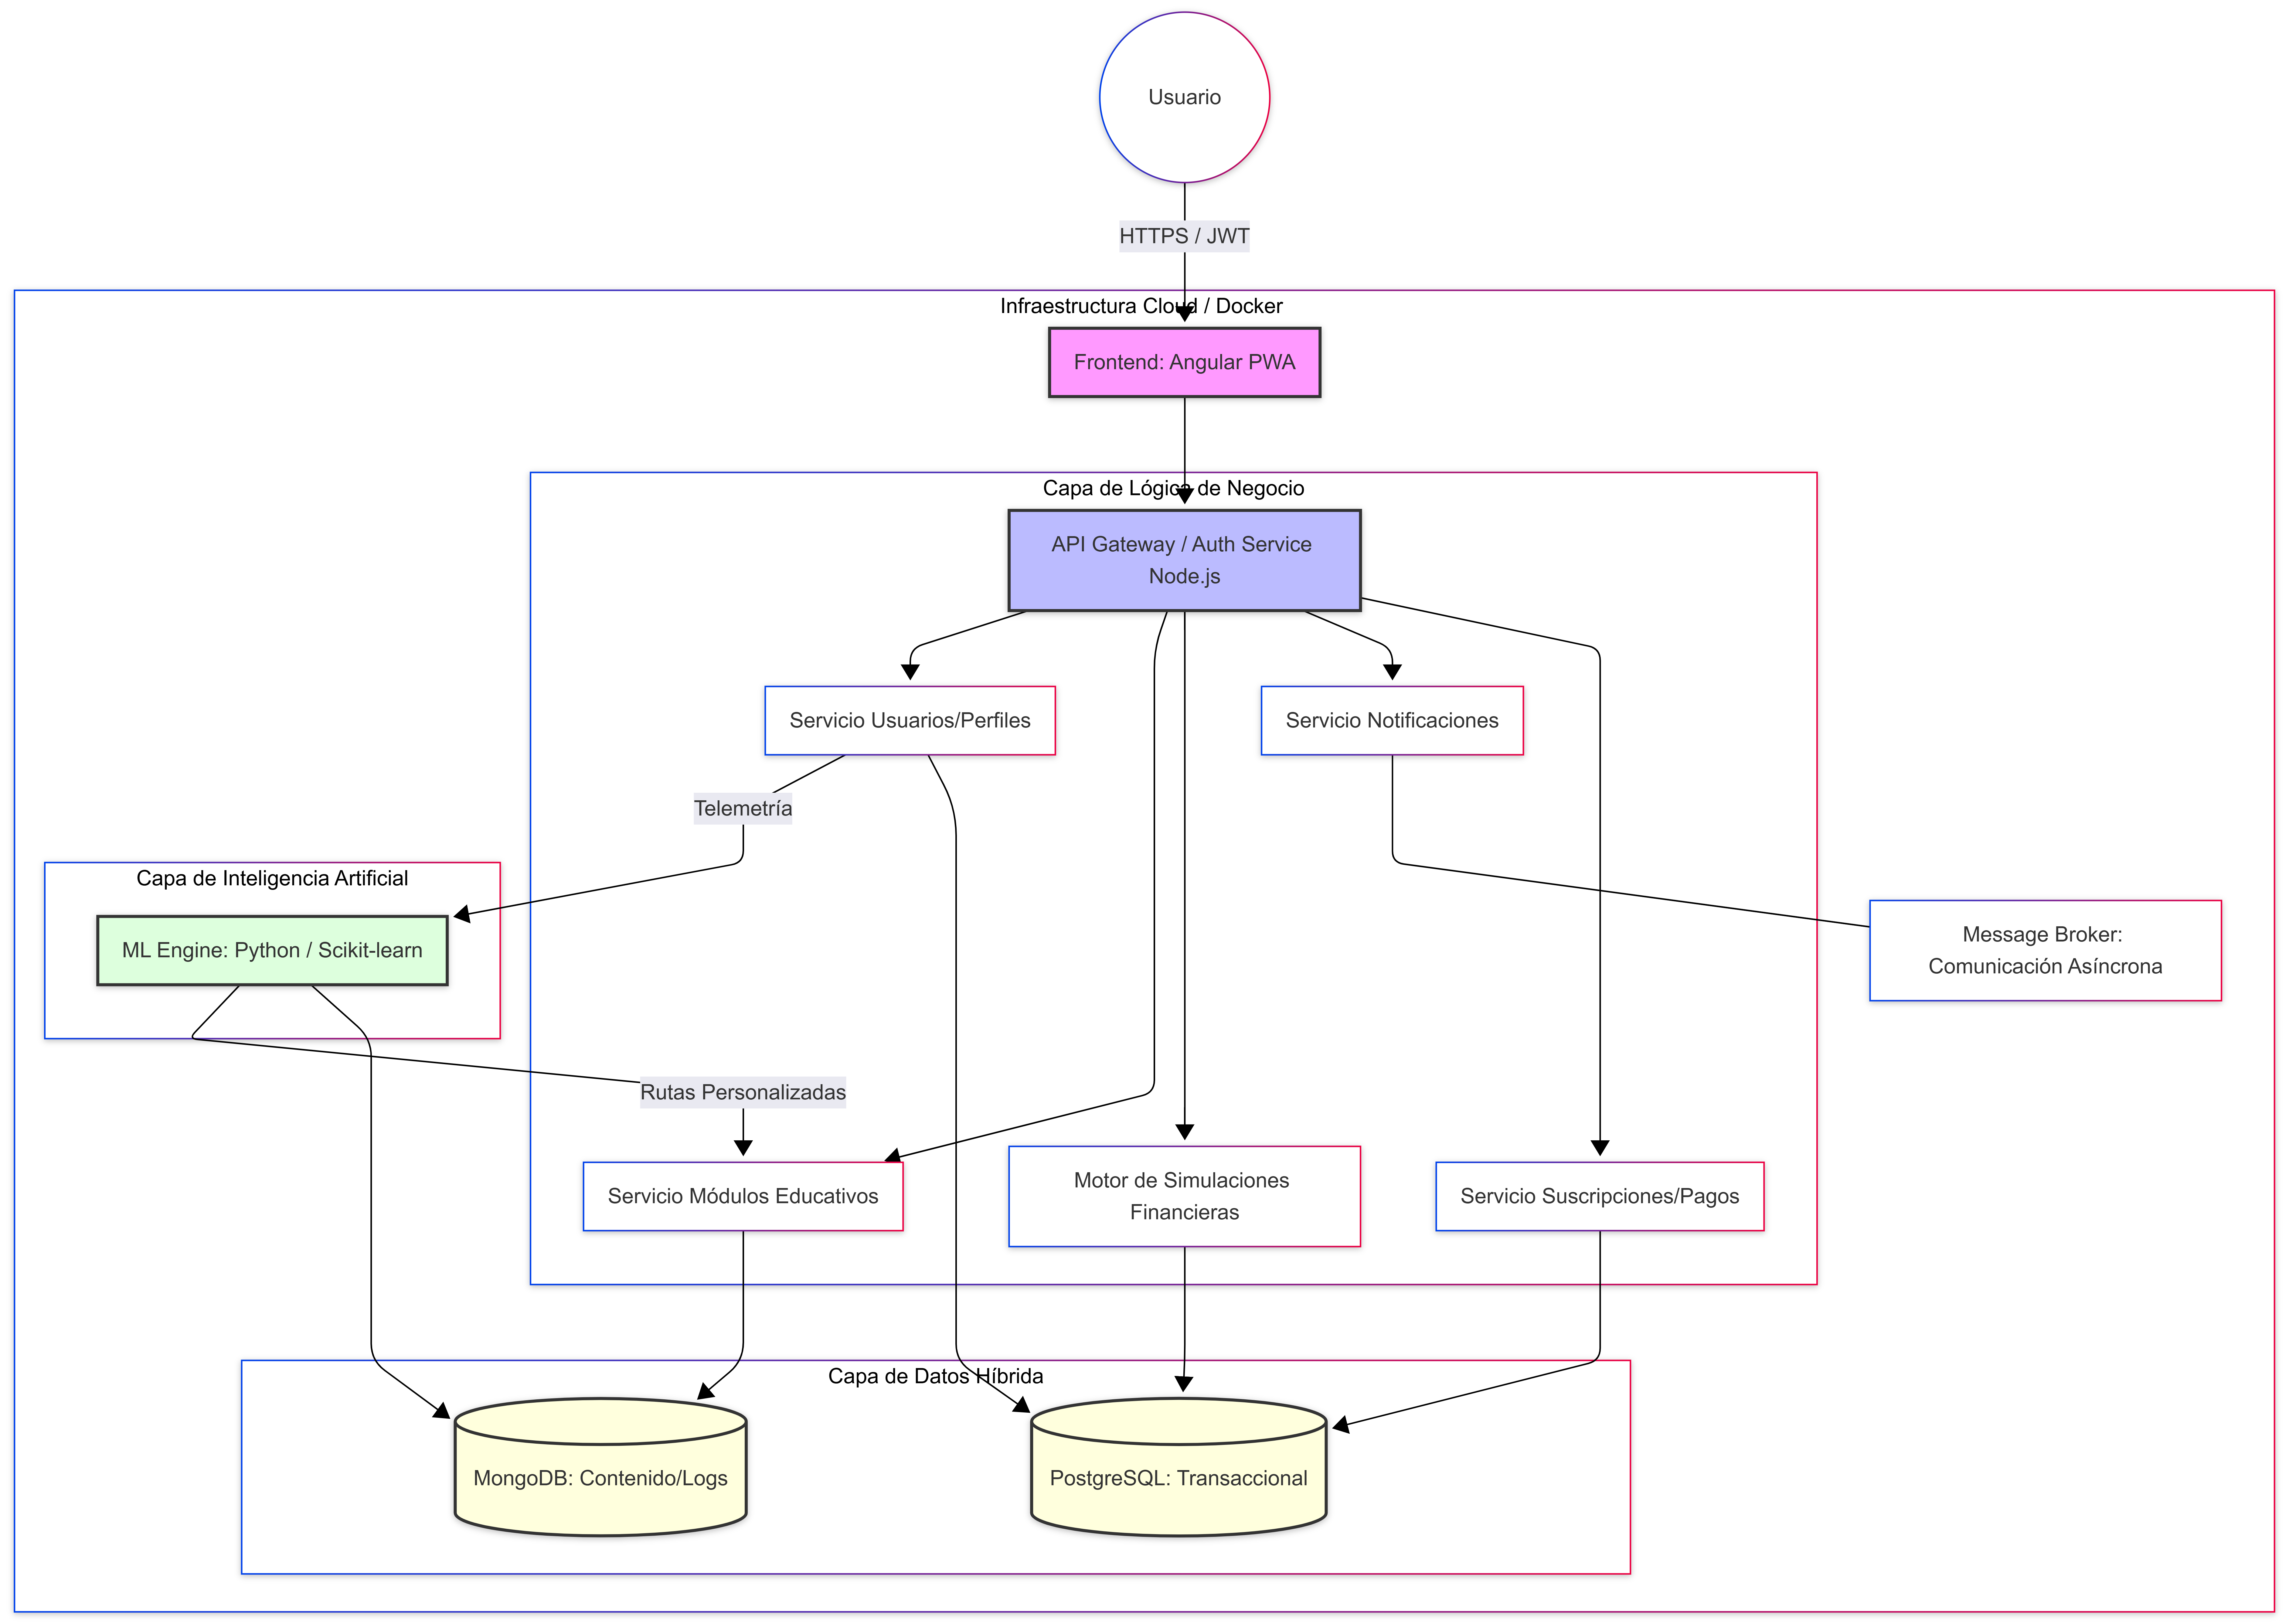
\includegraphics[width=0.85\textwidth]{Imagenes/arquitectura.png}
	\caption{Arquitectura Lógica de Microservicios de la Plataforma.}
	{\small \textit{Fuente:} Elaboración propia.}
	\label{fig:arquitectura_logica}
\end{figure}

\paragraph*{Diagrama de Despliegue de Infraestructura}
La distribución física del sistema, detallada en la Figura \ref{fig:despliegue_fisico}, se fundamenta en una estrategia de \textbf{contenerización} con Docker. Esta configuración garantiza que el sistema sea agnóstico respecto al proveedor de servicios de nube (\textit{Cloud Agnostic}), facilitando el despliegue en entornos como AWS, Azure o Google Cloud. Se destaca la inclusión de una \textbf{CDN} (Red de Distribución de Contenido) para optimizar la entrega de material multimedia en la región de Bogotá, cumpliendo con los estándares de rendimiento (RNF06).

\begin{figure}[H]
	\centering
	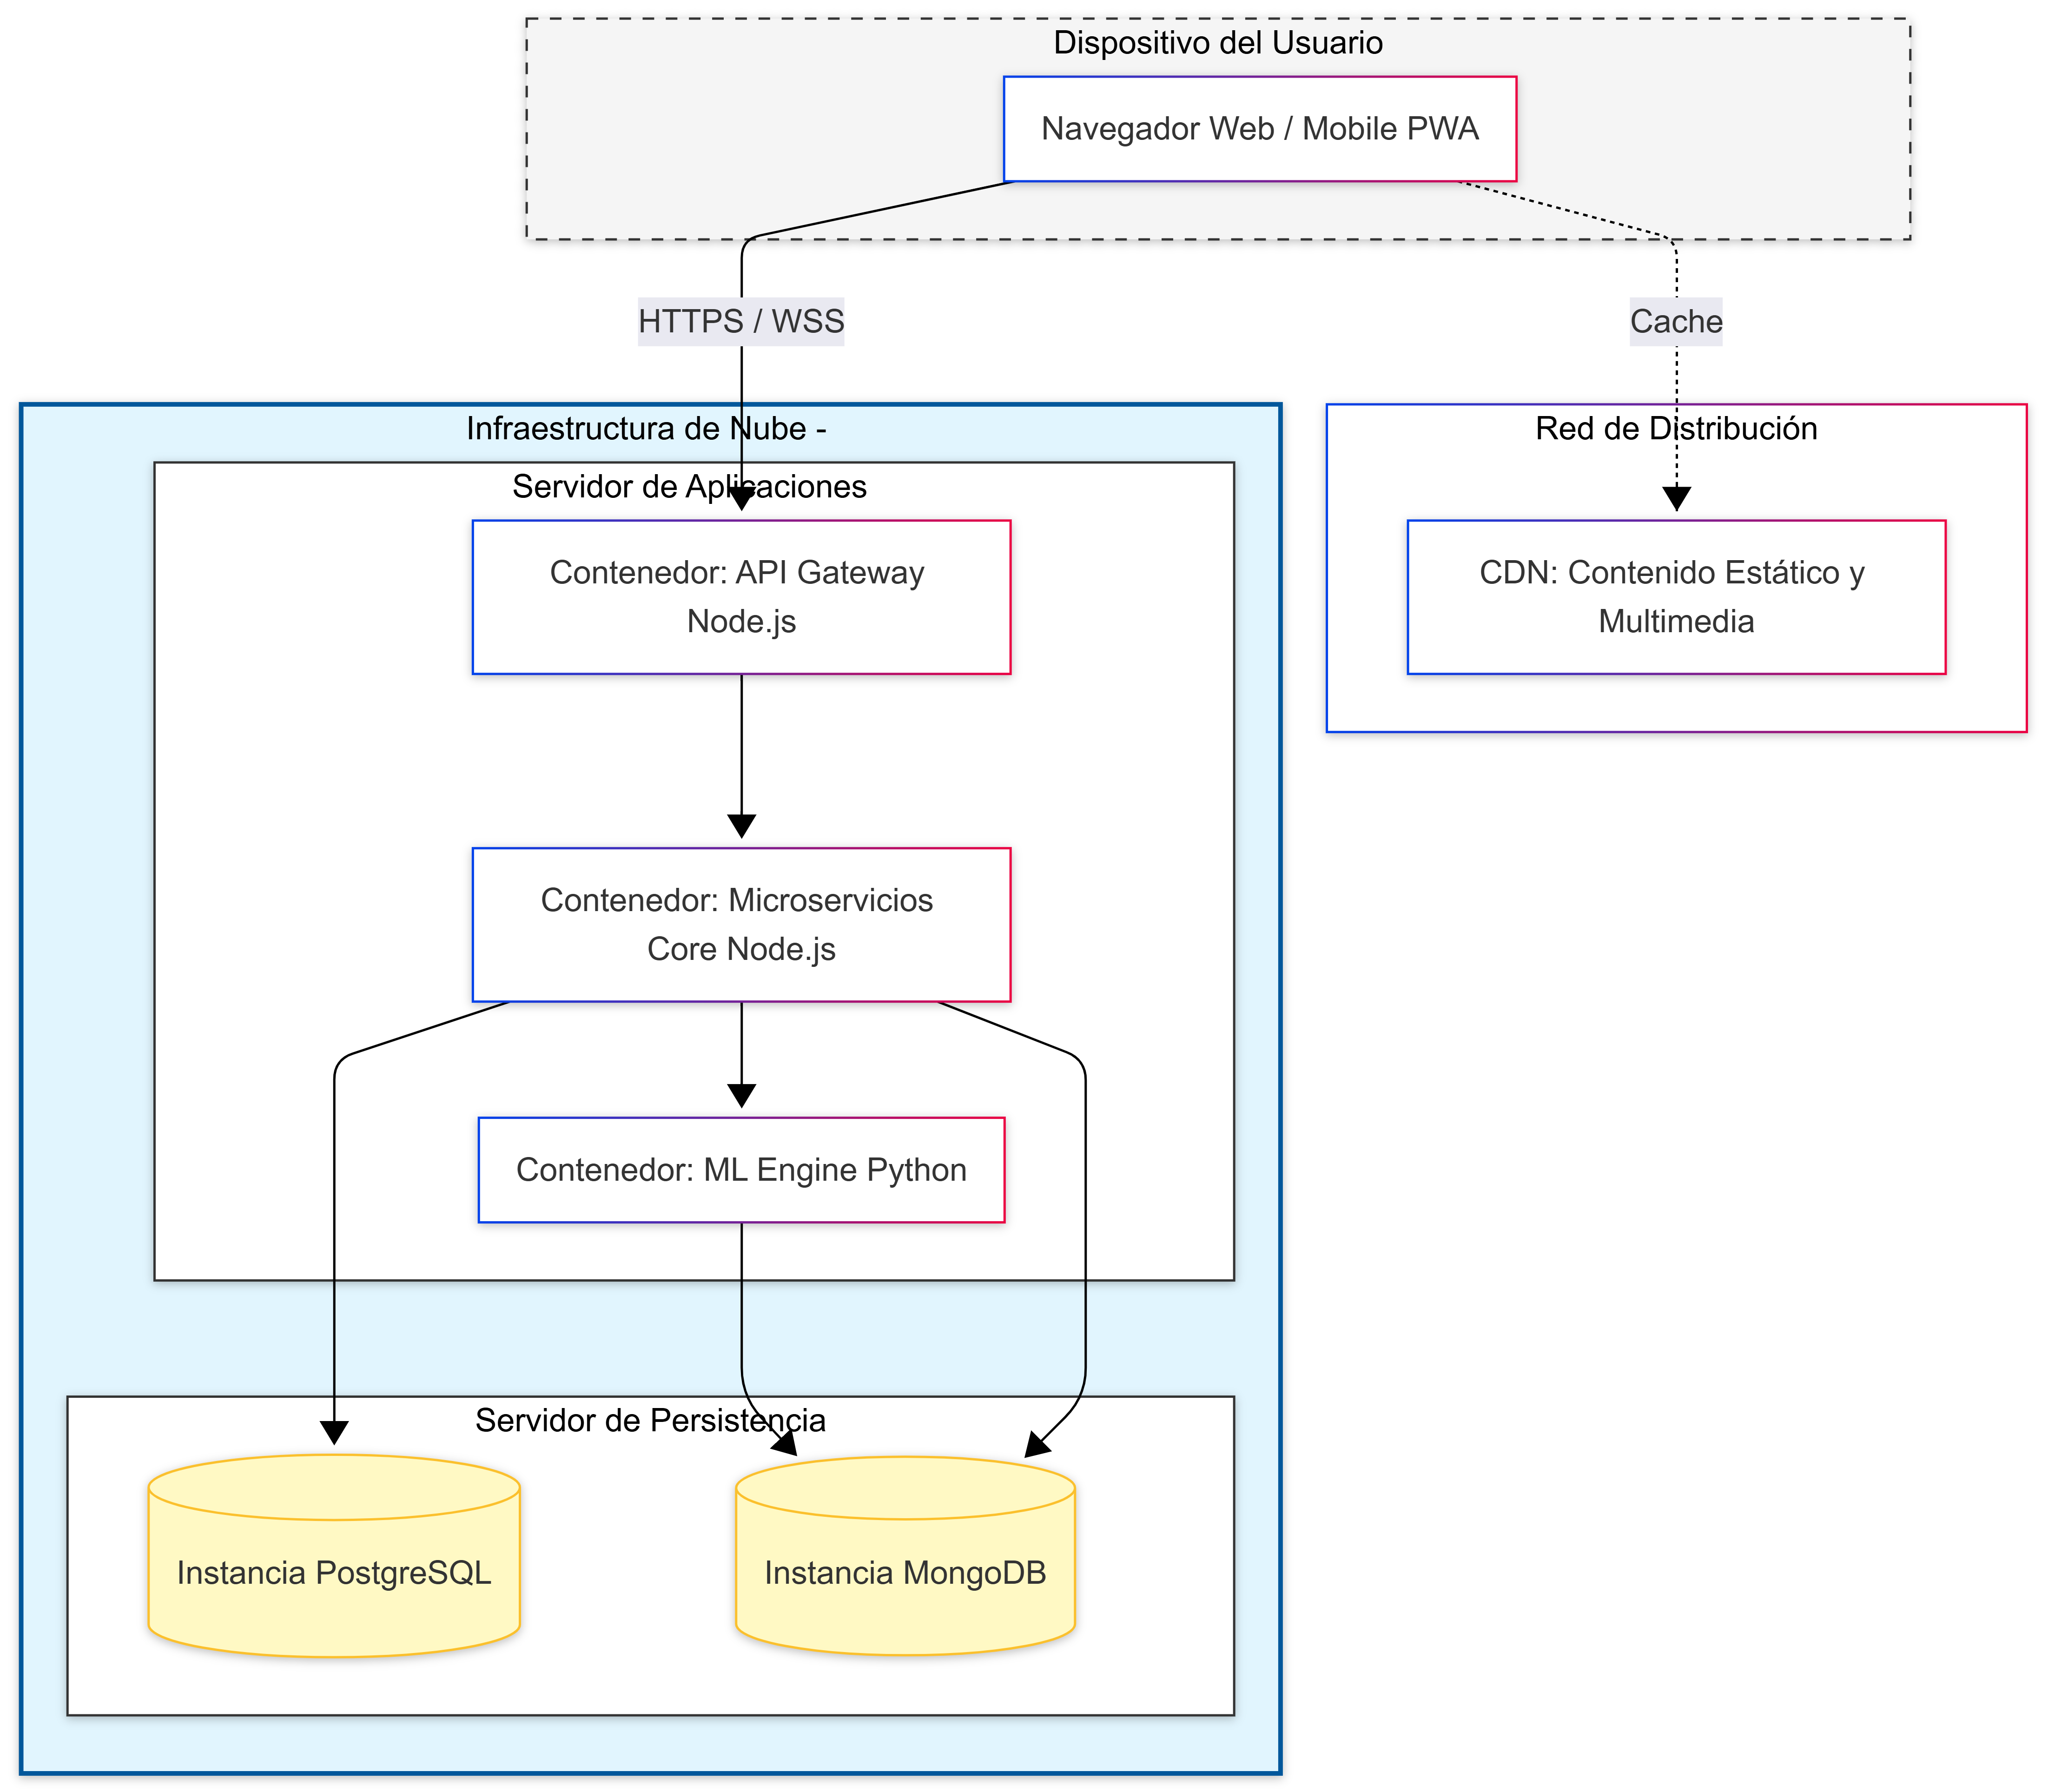
\includegraphics[width=0.85\textwidth]{Imagenes/despliegue.png}
	\caption{Diagrama de Despliegue de Infraestructura en la Nube.}
	{\small \textit{Fuente:} Elaboración propia.}
	\label{fig:despliegue_fisico}
\end{figure}

\phantomsection
\addcontentsline{toc}{subsubsection}{Tecnologías Seleccionadas}
\subsubsection*{Tecnologías Seleccionadas}

Para garantizar la viabilidad técnica del PMV, se han seleccionado herramientas que priorizan el alto rendimiento y la escalabilidad:

\begin{itemize}
	\item \textbf{Angular (Frontend):} Framework basado en TypeScript que permite una arquitectura modular y fluida, similar a los estándares de las aplicaciones bancarias actuales.
	\item \textbf{Node.js (Backend):} Entorno de ejecución basado en eventos que soporta una alta concurrencia de peticiones simultáneas sin bloqueos.
	\item \textbf{Python (IA/ML):} Lenguaje líder en ciencia de datos, utilizado para exponer los modelos de recomendación como servicios independientes.
	\item \textbf{Persistencia:} El uso dual de PostgreSQL y MongoDB permite equilibrar la seguridad de los datos financieros con la flexibilidad necesaria para los contenidos educativos.
\end{itemize}

Esta integración tecnológica asegura un ecosistema de desarrollo homogéneo bajo estándares de \textit{Clean Architecture}, facilitando la validación rápida de hipótesis bajo la metodología \textit{Lean Startup}.

\phantomsection
\addcontentsline{toc}{subsubsection}{Requerimientos}
\subsubsection*{Requerimientos}

A continuación, se especifican los requerimientos del sistema, los cuales establecen las capacidades funcionales y las restricciones de calidad que debe cumplir la plataforma para satisfacer los objetivos del proyecto.

\paragraph*{Requerimientos funcionales}
\addcontentsline{toc}{paragraph}{Requerimientos funcionales}
Los requerimientos funcionales describen las acciones específicas que debe realizar el sistema, estos requerimientos funcionales se describen a continuación:

\begin{table}[H]
	\begin{tabular}{|a{5cm}|m{11cm}|}
		\hline
		\textbf{Código} & RF01 \\ \hline
		\textbf{Nombre del requerimiento} & Registro de cuenta de usuarios \\ \hline
		\textbf{Fecha} & 15/10/2025 \\ \hline
		\textbf{Tipo de requerimiento} & Funcional \\ \hline
		\textbf{Origen de requerimiento} & Análisis del sistema \\ \hline
		\textbf{Prioridad} & Alta \\ \hline
		\textbf{Actor} & Usuario y administrador \\ \hline
		\textbf{Descripción} & El sistema debe permitir a los nuevos usuarios crear una cuenta mediante un formulario que capture nombre completo, correo electrónico y contraseña. El sistema debe validar que el correo no esté registrado previamente y cifrar la contraseña antes de almacenarla.\\ \hline
		\textbf{Criterio de aceptación} & Se crea un nuevo registro en la base de datos PostgreSQL y el sistema redirige al usuario al flujo de bienvenida o verificación de correo. \\ \hline
	\end{tabular}
\end{table}

\begin{table}[H]
	\begin{tabular}{|a{5cm}|m{11cm}|}
		\hline
		\textbf{Código} & RF02 \\ \hline
		\textbf{Nombre del requerimiento} & Autenticación y Control de Acceso \\ \hline
		\textbf{Fecha} & 15/10/2025 \\ \hline
		\textbf{Tipo de requerimiento} & Funcional \\ \hline
		\textbf{Origen de requerimiento} & Análisis del sistema \\ \hline
		\textbf{Prioridad} & Alta \\ \hline
		\textbf{Actor} & Usuario y administrador \\ \hline
		\textbf{Descripción} & El sistema debe validar las credenciales del usuario (email y contraseña) contra los registros existentes. Tras una validación exitosa, el backend debe generar un token de acceso (JWT) que permita al usuario consumir los servicios protegidos de la arquitectura de microservicios. \\ \hline
		\textbf{Criterio de aceptación} & El usuario accede a su sesión privada; en caso de credenciales inválidas, el sistema debe denegar el acceso y mostrar un mensaje de error genérico por seguridad. \\ \hline
	\end{tabular}
\end{table}

\begin{table}[H]
	\begin{tabular}{|a{5cm}|m{11cm}|}
		\hline
		\textbf{Código} & RF03 \\ \hline
		\textbf{Nombre del requerimiento} & Gestión y Caracterización de Perfil de Usuario \\ \hline
		\textbf{Fecha} & 15/10/2025 \\ \hline
		\textbf{Tipo de requerimiento} & Funcional \\ \hline
		\textbf{Origen de requerimiento} & Análisis del sistema \\ \hline
		\textbf{Prioridad} & Media \\ \hline
		\textbf{Actor} & Usuario y sistema \\ \hline
		\textbf{Descripción} & El sistema debe permitir al usuario completar y actualizar su información sociodemográfica y financiera básica (ingresos, metas, tipo de ocupación). Estos datos deben persistir para alimentar de forma dinámica el motor de recomendaciones. \\ \hline
		\textbf{Criterio de aceptación} & El perfil se guarda correctamente en PostgreSQL; los cambios se reflejan inmediatamente en la interfaz y quedan disponibles para el microservicio de Machine Learning. \\ \hline
	\end{tabular}
\end{table}

\begin{table}[H]
	\begin{tabular}{|a{5cm}|m{11cm}|}
		\hline
		\textbf{Código} & RF04 \\ \hline
		\textbf{Nombre del requerimiento} & Motor de Simulaciones Financieras Adaptativas \\ \hline
		\textbf{Fecha} & 15/10/2025 \\ \hline
		\textbf{Tipo de requerimiento} & Funcional \\ \hline
		\textbf{Origen de requerimiento} & Plan de negocio \\ \hline
		\textbf{Prioridad} & Alta \\ \hline
		\textbf{Actor} & Usuario \\ \hline
		\textbf{Descripción} & El sistema debe proveer herramientas de cálculo para ahorro, crédito e inversión. Debe procesar variables de entrada (capital, tiempo, tasa) y devolver proyecciones basadas en modelos financieros estandarizados. \\ \hline
		\textbf{Criterio de aceptación} & El motor de cálculo devuelve resultados con precisión decimal; los datos se visualizan mediante componentes gráficos interactivos en Angular. \\ \hline
	\end{tabular}
\end{table}


\begin{table}[H]
	\begin{tabular}{|a{5cm}|m{11cm}|}
		\hline
		\textbf{Código} & RF05 \\ \hline
		\textbf{Nombre del requerimiento} & Gestión de presupuesto y ahorro \\ \hline
		\textbf{Fecha} & 15/10/2025 \\ \hline
		\textbf{Tipo de requerimiento} & Funcional \\ \hline
		\textbf{Origen de requerimiento} & Estudio de usabilidad \\ \hline
		\textbf{Prioridad} & Media \\ \hline
		\textbf{Actor} & Usuario \\ \hline
		\textbf{Descripción} & Módulo para registrar ingresos y gastos con interfaz intuitiva e incentivos (puntos o insignias) al alcanzar metas de ahorro. \\ \hline
		\textbf{Criterio de aceptación} & El usuario añade o clasifica transacciones; la app actualiza totales y gráficos de presupuesto, y otorga recompensas al lograr metas definidas (ver perfil con puntos/insignias). \\ \hline
	\end{tabular}
\end{table}

\begin{table}[H]
	\begin{tabular}{|a{5cm}|m{11cm}|}
		\hline
		\textbf{Código} & RF06 \\ \hline
		\textbf{Nombre del requerimiento} & Servicio Automatizado de Notificaciones \\ \hline
		\textbf{Fecha} & 15/10/2025 \\ \hline
		\textbf{Tipo de requerimiento} & Funcional \\ \hline
		\textbf{Origen de requerimiento} & Análisis del sistema \\ \hline
		\textbf{Prioridad} & Media \\ \hline
		\textbf{Actor} & Usuario y sistema \\ \hline
		\textbf{Descripción} & El sistema debe programar y enviar alertas automáticas basadas en fechas de vencimiento de obligaciones financieras o proximidad al cumplimiento de metas de ahorro definidas por el usuario. \\ \hline
		\textbf{Criterio de aceptación} & El microservicio de notificaciones dispara la alerta en la fecha y hora configurada; el usuario recibe la notificación de manera asíncrona en la plataforma. \\ \hline
	\end{tabular}
\end{table}

\begin{table}[H]
	\begin{tabular}{|a{5cm}|m{11cm}|}
		\hline
		\textbf{Código} & RF07 \\ \hline
		\textbf{Nombre del requerimiento} & Adquisición de plan de suscripción \\ \hline
		\textbf{Fecha} & 15/10/2025 \\ \hline
		\textbf{Tipo de requerimiento} & Funcional \\ \hline
		\textbf{Origen de requerimiento} & Comercialización \\ \hline
		\textbf{Prioridad} & Alta \\ \hline
		\textbf{Actor} & Usuario \\ \hline
		\textbf{Descripción} & El sistema debe ofrecer al usuario la posiblidad de seleccionar y suscribirse a la plataforma, ofreciendo un mayor número de características y menores límites. \\ \hline
		\textbf{Criterio de aceptación} & El usuario puede seleccionar y adquirir la suscripción directamente desde el sistema, con un proceso de pago en línea exitoso y confirmando la suscripción. \\ \hline
	\end{tabular}
\end{table}

\begin{table}[H]
	\begin{tabular}{|a{5cm}|m{11cm}|}
		\hline
		\textbf{Código} & RF08 \\ \hline
		\textbf{Nombre del requerimiento} & Motor de Personalización (Machine Learning) \\ \hline
		\textbf{Fecha} & 15/10/2025 \\ \hline
		\textbf{Tipo de requerimiento} & Funcional \\ \hline
		\textbf{Origen de requerimiento} & Plan de negocio \\ \hline
		\textbf{Prioridad} & Alta \\ \hline
		\textbf{Actor} & Usuario y sistema\\ \hline
		\textbf{Descripción} & Implementación de un microservicio en Python que analice el perfil del usuario y sugiera una ruta de aprendizaje personalizada (módulos educativos y metas de ahorro). \\ \hline
		\textbf{Criterio de aceptación} & El sistema debe generar al menos tres recomendaciones de contenido basadas en los datos de entrada del usuario con una latencia de respuesta inferior a 2 segundos. \\ \hline
	\end{tabular}
\end{table}

\begin{table}[H]
	\begin{tabular}{|a{5cm}|m{11cm}|}
		\hline
		\textbf{Código} & RF09 \\ \hline
		\textbf{Nombre del requerimiento} & Visualización y Consumo de Módulos Educativos \\ \hline
		\textbf{Fecha} & 15/10/2025 \\ \hline
		\textbf{Tipo de requerimiento} & Funcional \\ \hline
		\textbf{Origen de requerimiento} & Plan de negocio \\ \hline
		\textbf{Prioridad} & Alta \\ \hline
		\textbf{Actor} & Usuario \\ \hline
		\textbf{Descripción} & El sistema debe presentar los módulos de aprendizaje financiero (texto, video, cuestionarios) organizados por categorías o según la ruta personalizada generada por la IA. \\ \hline
		\textbf{Criterio de aceptación} & El usuario puede acceder al contenido, marcar módulos como completados y visualizar su progreso en la barra de avance de la plataforma. \\ \hline
	\end{tabular}
\end{table}

\begin{table}[H]
	\begin{tabular}{|a{5cm}|m{11cm}|}
		\hline
		\textbf{Código} & RF10 \\ \hline
		\textbf{Nombre del requerimiento} & Panel de Administración de Contenidos y Usuarios \\ \hline
		\textbf{Fecha} & 15/10/2025 \\ \hline
		\textbf{Tipo de requerimiento} & Funcional \\ \hline
		\textbf{Origen de requerimiento} & Análisis del sistema \\ \hline
		\textbf{Prioridad} & Media \\ \hline
		\textbf{Actor} & Administrador \\ \hline
		\textbf{Descripción} & El sistema debe proveer una interfaz para que el administrador gestione usuarios, actualice las tasas de interés de referencia para los simuladores y cargue nuevo material educativo. \\ \hline
		\textbf{Criterio de aceptación} & Las actualizaciones realizadas en el panel se reflejan en la base de datos y afectan globalmente el comportamiento de los simuladores y módulos educativos. \\ \hline
	\end{tabular}
\end{table}

\begin{table}[H]
	\begin{tabular}{|a{5cm}|m{11cm}|}
		\hline
		\textbf{Código} & RF11 \\ \hline
		\textbf{Nombre del requerimiento} & Finalización de Sesión (Logout) \\ \hline
		\textbf{Fecha} & 15/10/2025 \\ \hline
		\textbf{Tipo de requerimiento} & Funcional \\ \hline
		\textbf{Origen de requerimiento} & Análisis del sistema \\ \hline
		\textbf{Prioridad} & Alta \\ \hline
		\textbf{Actor} & Usuario y Administrador \\ \hline
		\textbf{Descripción} & El sistema debe permitir el cierre de sesión voluntario, invalidando el token JWT en el cliente y redirigiendo al usuario a la interfaz pública de la plataforma. \\ \hline
		\textbf{Criterio de aceptación} & El token se elimina del almacenamiento local; cualquier intento posterior de acceder a rutas protegidas (/dashboard, /perfil) es rechazado por el sistema. \\ \hline
	\end{tabular}
\end{table}


\phantomsection
\addcontentsline{toc}{paragraph}{Requerimientos no funcionales}
\paragraph*{Requerimientos no funcionales}

Los requerimientos no funcionales describen las cualidades y estándares que debe tener el sistema, su comportamiento, y otros aspectos. Estos requerimientos no funcionales se describen a continuación:

\begin{table}[H]
	\begin{tabular}{|s{5cm}|m{11cm}|}
		\hline
		\textbf{Código} & RNF01 \\ \hline
		\textbf{Nombre del requerimiento} & Compatibilidad multiplataforma \\ \hline
		\textbf{Fecha} & 15/10/2025 \\ \hline
		\textbf{Tipo de requerimiento} & No funcional \\ \hline
		\textbf{Origen de requerimiento} & Tendencias tecnológicas \\ \hline
		\textbf{Prioridad} & Alta \\ \hline
		\textbf{Descripción} & La plataforma debe ser accesible mediante navegadores web modernos (Chrome, Firefox, Safari, Edge) y presentar un diseño responsivo que se adapte a dispositivos móviles y de escritorio. \\ \hline
		\textbf{Criterio de aceptación} & Visualización correcta en resoluciones desde 360px hasta 1920px de ancho; cumplimiento de estándares HTML5 y CSS3 comprobado mediante validadores. \\ \hline
	\end{tabular}
\end{table}

\begin{table}[H]
	\begin{tabular}{|s{5cm}|m{11cm}|}
		\hline
		\textbf{Código} & RNF02 \\ \hline
		\textbf{Nombre del requerimiento} & Usabilidad y Experiencia de Usuario (UX) \\ \hline
		\textbf{Fecha} & 15/10/2025 \\ \hline
		\textbf{Tipo de requerimiento} & No funcional \\ \hline
		\textbf{Origen de requerimiento} & Estudio de usabilidad \\ \hline
		\textbf{Prioridad} & Alta \\ \hline
		\textbf{Descripción} & La interfaz debe minimizar la carga cognitiva del usuario, permitiendo que las funciones de simulación y registro sean intuitivas sin necesidad de manuales externos. \\ \hline
		\textbf{Criterio de aceptación} & En pruebas de usuario, el 85\% de los participantes debe completar el flujo de simulación en menos de 3 minutos sin asistencia técnica \\ \hline
	\end{tabular}
\end{table}

\begin{table}[H]
	\begin{tabular}{|s{5cm}|m{11cm}|}
		\hline
		\textbf{Código} & RNF03 \\ \hline
		\textbf{Nombre del requerimiento} & Control de Acceso Basado en Roles (RBAC) \\ \hline
		\textbf{Fecha} & 15/10/2025 \\ \hline
		\textbf{Tipo de requerimiento} & No funcional \\ \hline
		\textbf{Origen de requerimiento} & Gestión de usuarios \\ \hline
		\textbf{Prioridad} & Alta \\ \hline
		\textbf{Descripción} & El sistema debe implementar una matriz de permisos que restrinja o habilite funciones según el rol asignado (Administrador, Premium, Gratuito) mediante tokens de sesión. \\ \hline
		\textbf{Criterio de aceptación} & El API Gateway rechaza peticiones de usuarios sin el rol adecuado (Error 403 Forbidden); los menús de la interfaz se ocultan dinámicamente según el perfil. \\ \hline
	\end{tabular}
\end{table}

\begin{table}[H]
	\begin{tabular}{|s{5cm}|m{11cm}|}
		\hline
		\textbf{Código} & RNF04 \\ \hline
		\textbf{Nombre del requerimiento} & Seguridad de la información y cifrado \\ \hline
		\textbf{Fecha} & 15/10/2025 \\ \hline
		\textbf{Tipo de requerimiento} & No funcional \\ \hline
		\textbf{Origen de requerimiento} & Normativa legal de seguridad \\ \hline
		\textbf{Prioridad} & Alta \\ \hline
		\textbf{Descripción} & Cifrado de datos en tránsito utilizando TLS 1.3 y cifrado de datos sensibles en reposo (AES-256). Las contraseñas deben procesarse con algoritmos de hashing robustos. \\ \hline
		\textbf{Criterio de aceptación} & Certificado SSL válido con calificación A en SSL Labs; verificación de que no existen textos planos de contraseñas en la base de datos PostgreSQL. \\ \hline
	\end{tabular}
\end{table}

\begin{table}[H]
	\begin{tabular}{|s{5cm}|m{11cm}|}
		\hline
		\textbf{Código} & RNF05 \\ \hline
		\textbf{Nombre del requerimiento} & Privacidad y Tratamiento de Datos Personales \\ \hline
		\textbf{Fecha} & 15/10/2025 \\ \hline
		\textbf{Tipo de requerimiento} & No funcional \\ \hline
		\textbf{Origen de requerimiento} &Ley 1581 de 2012 (Habeas Data) \\ \hline
		\textbf{Prioridad} & Alta \\ \hline
		\textbf{Descripción} & El sistema debe garantizar que el almacenamiento y procesamiento de datos financieros cumpla con la normativa colombiana de protección de datos personales. \\ \hline
		\textbf{Criterio de aceptación} & Firma digital de términos y condiciones en el registro; logs de auditoría que registren el acceso a datos sensibles. \\ \hline
	\end{tabular}
\end{table}

\begin{table}[H]
	\begin{tabular}{|s{5cm}|m{11cm}|}
		\hline
		\textbf{Código} & RNF06 \\ \hline
		\textbf{Nombre del requerimiento} & Rendimiento y tiempos e respuesta \\ \hline
		\textbf{Fecha} & 15/10/2025 \\ \hline
		\textbf{Tipo de requerimiento} & No funcional \\ \hline
		\textbf{Origen de requerimiento} & Experiencia de usuario \\ \hline
		\textbf{Prioridad} & Media \\ \hline
		\textbf{Descripción} & Las consultas al motor de simulaciones y la carga de datos del dashboard deben optimizarse para garantizar una respuesta fluida. \\ \hline
		\textbf{Criterio de aceptación} & Tiempo de respuesta del servidor (TTFB) menor a 500ms; carga total de la página principal en menos de 2.5 segundos bajo condiciones de red estándar. \\ \hline
	\end{tabular}
\end{table}

\begin{table}[H]
	\begin{tabular}{|s{5cm}|m{11cm}|}
		\hline
		\textbf{Código} & RNF07 \\ \hline
		\textbf{Nombre del requerimiento} & Disponibilidad y confiabilidad \\ \hline
		\textbf{Fecha} & 15/10/2025 \\ \hline
		\textbf{Tipo de requerimiento} & No funcional \\ \hline
		\textbf{Origen de requerimiento} & Acuerdo de Nivel de Servicio (SLA) \\ \hline
		\textbf{Prioridad} & Media \\ \hline
		\textbf{Descripción} & El sistema debe mantener una disponibilidad del 99.5\% mensual. Se deben realizar respaldos automáticos diarios de la base de datos con una política de retención de 30 días. \\ \hline
		\textbf{Criterio de aceptación} & Reportes de monitoreo mensual sin caídas superiores a 3.6 horas; ejecución verificada de scripts de backup en contenedores Docker. \\ \hline
	\end{tabular}
\end{table}

\begin{table}[H]
	\begin{tabular}{|s{5cm}|m{11cm}|}
		\hline
		\textbf{Código} & RNF08 \\ \hline
		\textbf{Nombre del requerimiento} & Accesibilidad \\ \hline
		\textbf{Fecha} & 15/10/2025 \\ \hline
		\textbf{Tipo de requerimiento} & No funcional \\ \hline
		\textbf{Origen de requerimiento} & Requerimientos de accesibilidad \\ \hline
		\textbf{Prioridad} & Media \\ \hline
		\textbf{Descripción} & Cumplir estándares básicos (p.ej. WCAG 2.1 AA): contraste adecuado, etiquetas en controles, navegación compatible con lectores de pantalla. \\ \hline
		\textbf{Criterio de aceptación} & Verificación WCAG: textos legibles y contrastados, elementos interactivos etiquetados. Se confirma funcionalidad con un lector de pantalla. \\ \hline
	\end{tabular}
\end{table}

\begin{table}[H]
	\begin{tabular}{|s{5cm}|m{11cm}|}
		\hline
		\textbf{Código} & RNF09 \\ \hline
		\textbf{Nombre del requerimiento} & Mantenibilidad y documentación técnica\\ \hline
		\textbf{Fecha} & 15/10/2025 \\ \hline
		\textbf{Tipo de requerimiento} & No funcional \\ \hline
		\textbf{Origen de requerimiento} & Buenas prácticas de desarrollo \\ \hline
		\textbf{Prioridad} & Media \\ \hline
		\textbf{Descripción} & El código fuente debe seguir patrones de diseño modulares (Clean Architecture) y contar con documentación técnica exhaustiva para facilitar el mantenimiento preventivo y correctivo.. \\ \hline
		\textbf{Criterio de aceptación} & Repositorio con README detallado, comentarios en funciones críticas y cobertura de pruebas unitarias superior al 70\% \\ \hline
	\end{tabular}
\end{table}

\begin{table}[H]
	\begin{tabular}{|s{5cm}|m{11cm}|}
		\hline
		\textbf{Código} & RNF10 \\ \hline
		\textbf{Nombre del requerimiento} & Escalabilidad \\ \hline
		\textbf{Fecha} & 15/10/2025 \\ \hline
		\textbf{Tipo de requerimiento} & No funcional \\ \hline
		\textbf{Origen de requerimiento} & Plan de Negocio e infraestructura \\ \hline
		\textbf{Prioridad} & Baja \\ \hline
		\textbf{Descripción} & La infraestructura basada en microservicios y contenedores debe permitir el despliegue de múltiples instancias para absorber picos de tráfico sin degradación del servicio. \\ \hline
		\textbf{Criterio de aceptación} & El sistema soporta un incremento de hasta 500 usuarios concurrentes mediante el escalado de pods en el clúster sin aumentar los tiempos de respuesta por encima de 1s. \\ \hline
	\end{tabular}
\end{table}

\phantomsection
\addcontentsline{toc}{subsubsection}{Casos de uso}
\subsubsection*{Casos de uso}

Los casos de uso describen detalladamente cómo un usuario interactúa con nuestro sistema para alcanzar un objetivo, a continuación, mostramos los casos de usos para los requerimientos funcionales dados anteriormente:

\begin{figure}[H]
	\centering
	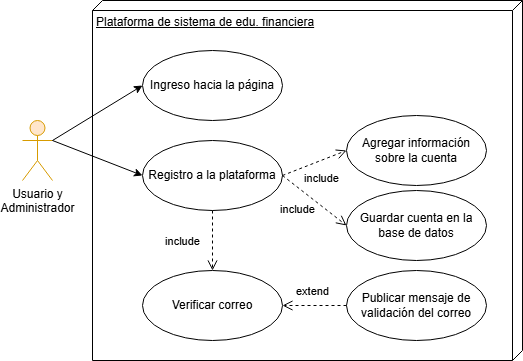
\includegraphics[width=12cm]{Imagenes/CasoUsoRF01.png}
	\caption[{Diagrama de caso de uso RF01.}]{\centering Diagrama de caso de uso RF01. \textit{Fuente:} Autores.}
	\label{fig:diagramacasousorf01}
\end{figure}

\begin{figure}[H]
	\centering
	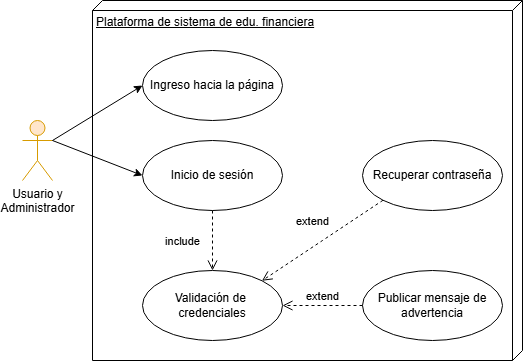
\includegraphics[width=12cm]{Imagenes/CasoUsoRF02.png}
	\caption[{Diagrama de caso de uso RF02.}]{\centering Diagrama de caso de uso RF02. \textit{Fuente:} Autores.}
	\label{fig:diagramacasousorf02}
\end{figure}

\begin{figure}[H]
	\centering
	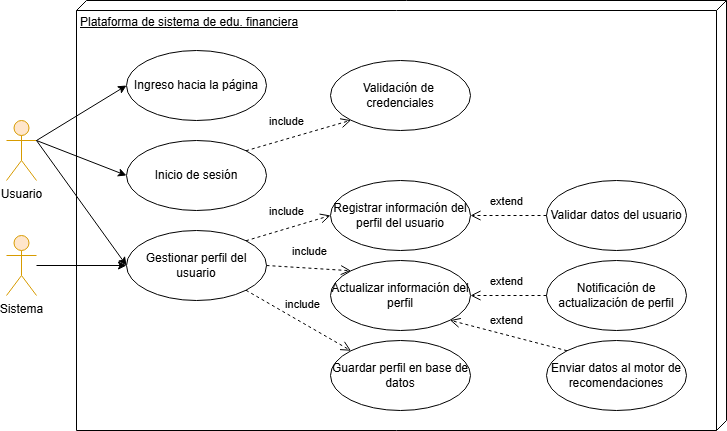
\includegraphics[width=12cm]{Imagenes/CasoUsoRF03.png}
	\caption[{Diagrama de caso de uso RF03.}]{\centering Diagrama de caso de uso RF03. \textit{Fuente:} Autores.}
	\label{fig:diagramacasousorf03}
\end{figure}

\begin{figure}[H]
	\centering
	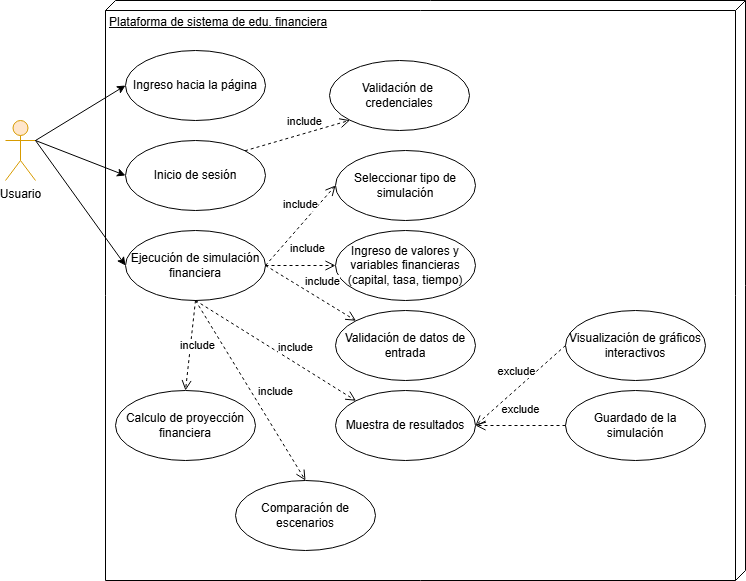
\includegraphics[width=12cm]{Imagenes/CasoUsoRF04.png}
	\caption[{Diagrama de caso de uso RF04.}]{\centering Diagrama de caso de uso RF04. \textit{Fuente:} Autores.}
	\label{fig:diagramacasousorf04}
\end{figure}

\begin{figure}[H]
	\centering
	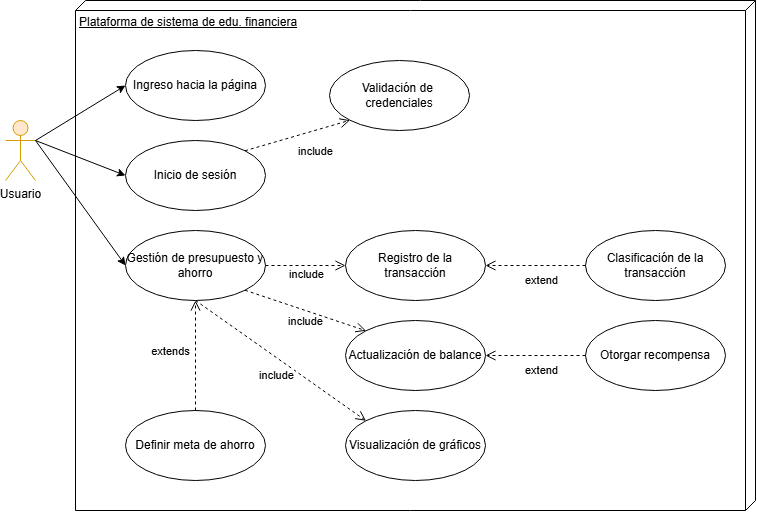
\includegraphics[width=12cm]{Imagenes/CasoUsoRF05.png}
	\caption[{Diagrama de caso de uso RF05.}]{\centering Diagrama de caso de uso RF05. \textit{Fuente:} Autores.}
	\label{fig:diagramacasousorf05}
\end{figure}

\begin{figure}[H]
	\centering
	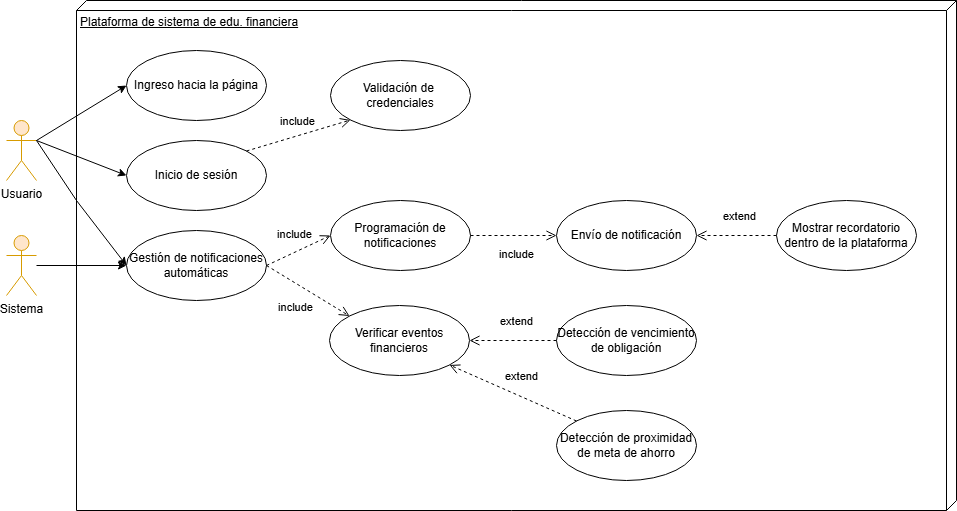
\includegraphics[width=12cm]{Imagenes/CasoUsoRF06.png}
	\caption[{Diagrama de caso de uso RF06.}]{\centering Diagrama de caso de uso RF06. \textit{Fuente:} Autores.}
	\label{fig:diagramacasousorf06}
\end{figure}

\begin{figure}[H]
	\centering
	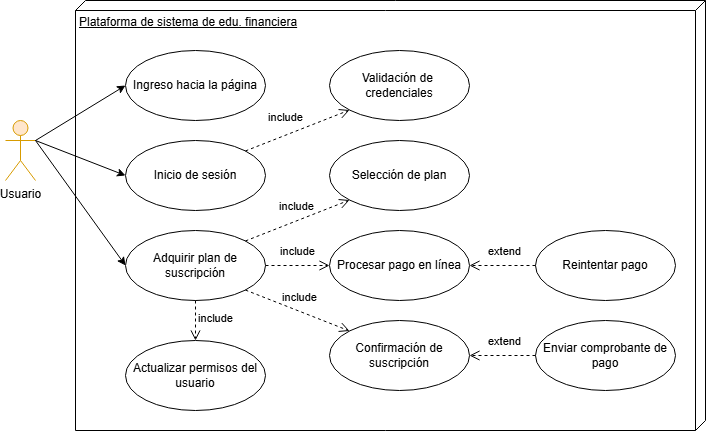
\includegraphics[width=12cm]{Imagenes/CasoUsoRF07.png}
	\caption[{Diagrama de caso de uso RF07.}]{\centering Diagrama de caso de uso RF07. \textit{Fuente:} Autores.}
	\label{fig:diagramacasousorf07}
\end{figure}

\begin{figure}[H]
	\centering
	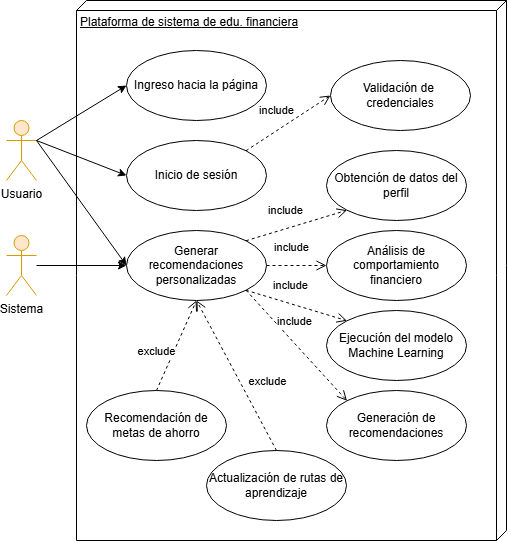
\includegraphics[width=12cm]{Imagenes/CasoUsoRF08.png}
	\caption[{Diagrama de caso de uso RF08.}]{\centering Diagrama de caso de uso RF08. \textit{Fuente:} Autores.}
	\label{fig:diagramacasousorf08}
\end{figure}

\begin{figure}[H]
	\centering
	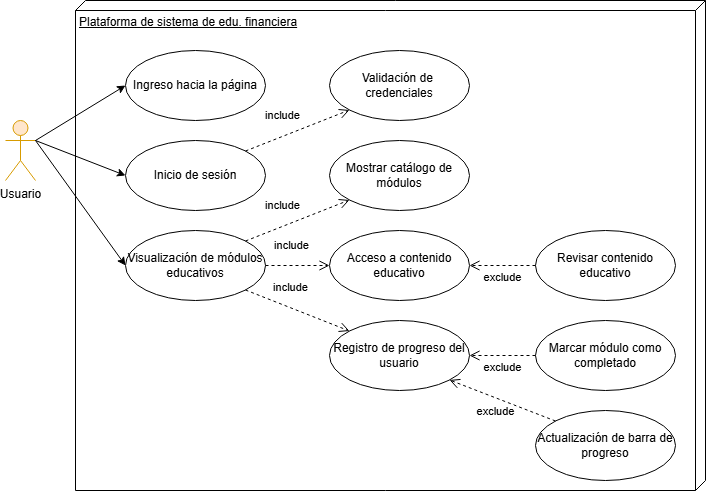
\includegraphics[width=12cm]{Imagenes/CasoUsoRF09.png}
	\caption[{Diagrama de caso de uso RF09.}]{\centering Diagrama de caso de uso RF09. \textit{Fuente:} Autores.}
	\label{fig:diagramacasousorf09}
\end{figure}

\begin{figure}[H]
	\centering
	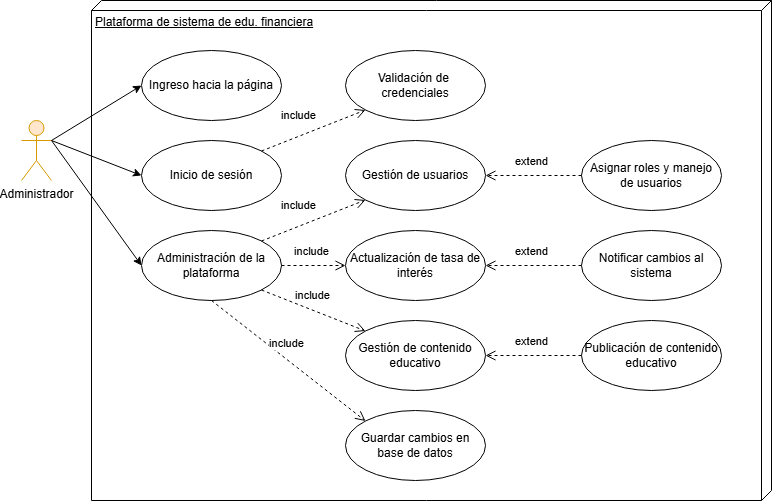
\includegraphics[width=12cm]{Imagenes/CasoUsoRF10.png}
	\caption[{Diagrama de caso de uso RF10.}]{\centering Diagrama de caso de uso RF10. \textit{Fuente:} Autores.}
	\label{fig:diagramacasousorf10}
\end{figure}

\begin{figure}[H]
	\centering
	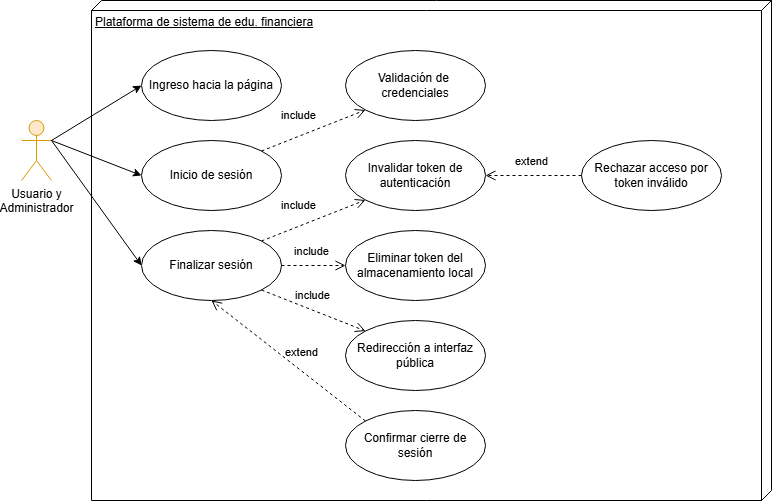
\includegraphics[width=12cm]{Imagenes/CasoUsoRF11.png}
	\caption[{Diagrama de caso de uso RF11.}]{\centering Diagrama de caso de uso RF11. \textit{Fuente:} Autores.}
	\label{fig:diagramacasousorf11}
\end{figure}

\phantomsection
\addcontentsline{toc}{subsubsection}{Vistas principales del prototipo}
\subsubsection*{Vistas principales del prototipo}


Concorde a lo previamente descrito dentro de las historias de usuario y los casos de uso, se adjunta algunas vistas base del prototipo. Cabe aclarar que las siguientes ilustraciones para diseñar el modelo fueron obtenidas del sitio en el que esta ubicado el producto mínimo viable.

\begin{figure}[H]
	\centering
	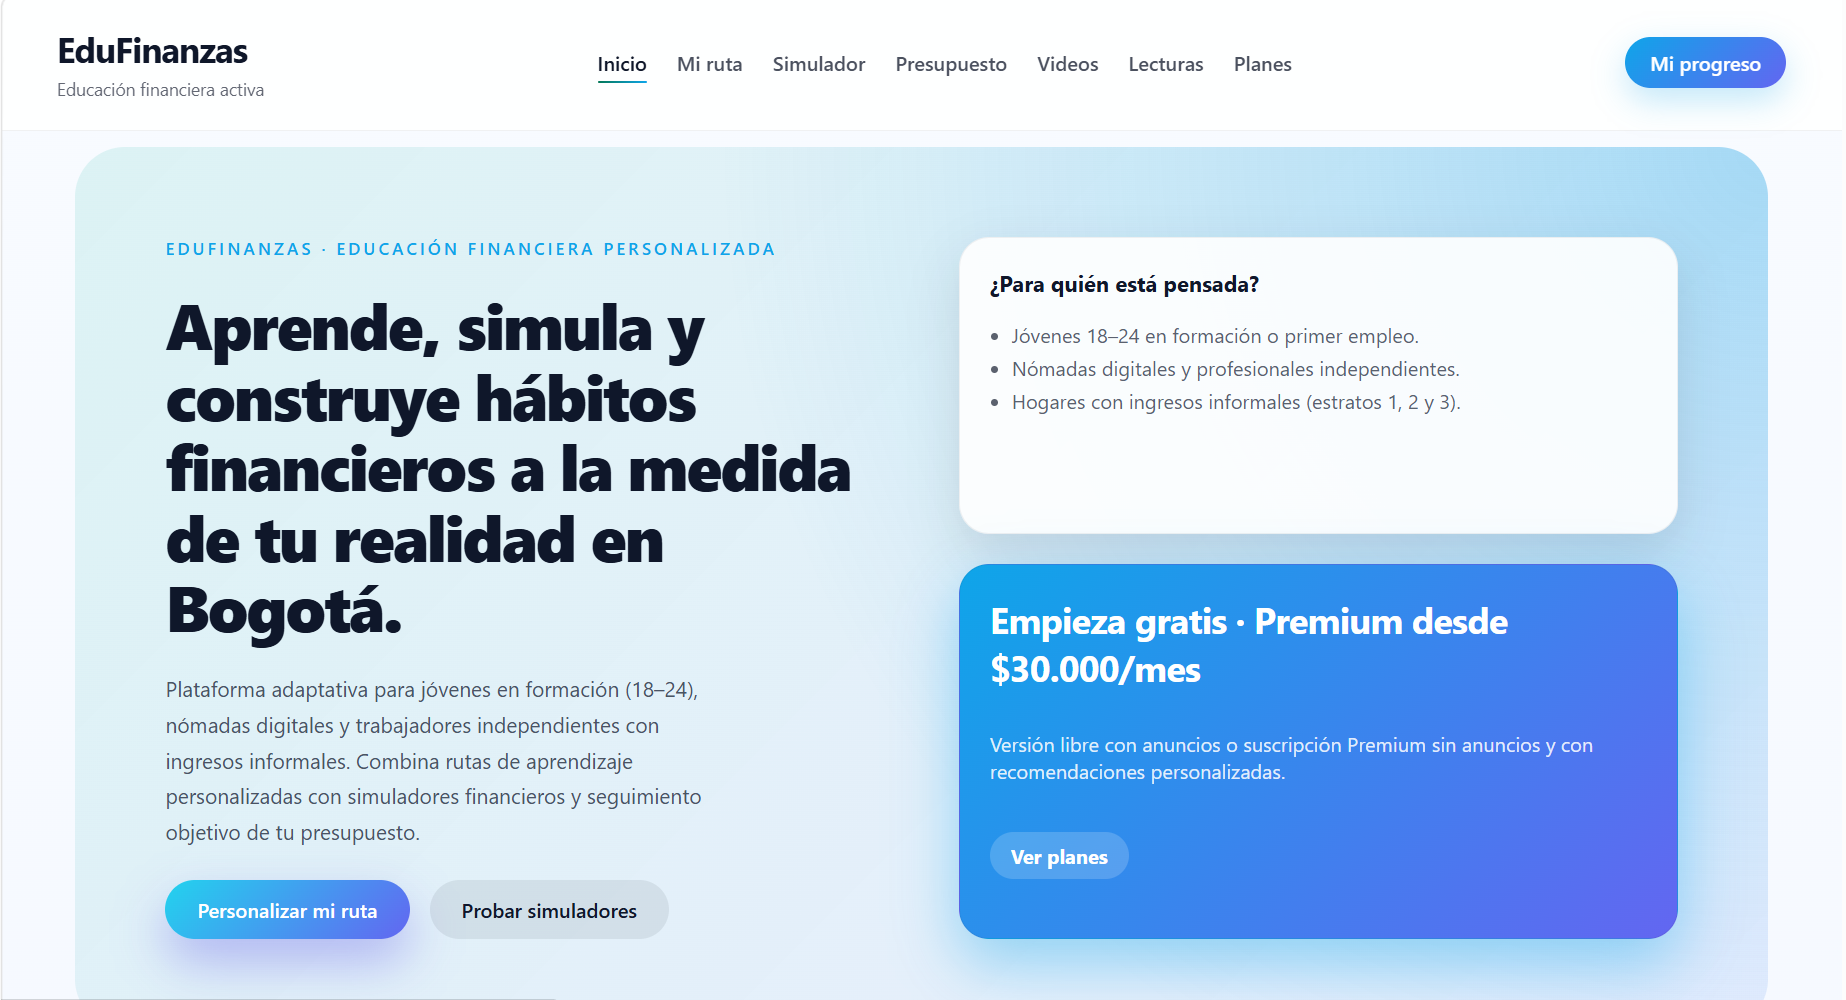
\includegraphics[width=15cm]{Imagenes/principal.png}
	\caption[{Vista principal.}]{\centering Vista principal. \textit{Fuente:} Autores.}
	\label{fig:vistaprincipal}
\end{figure}

\begin{figure}[H]
	\centering
	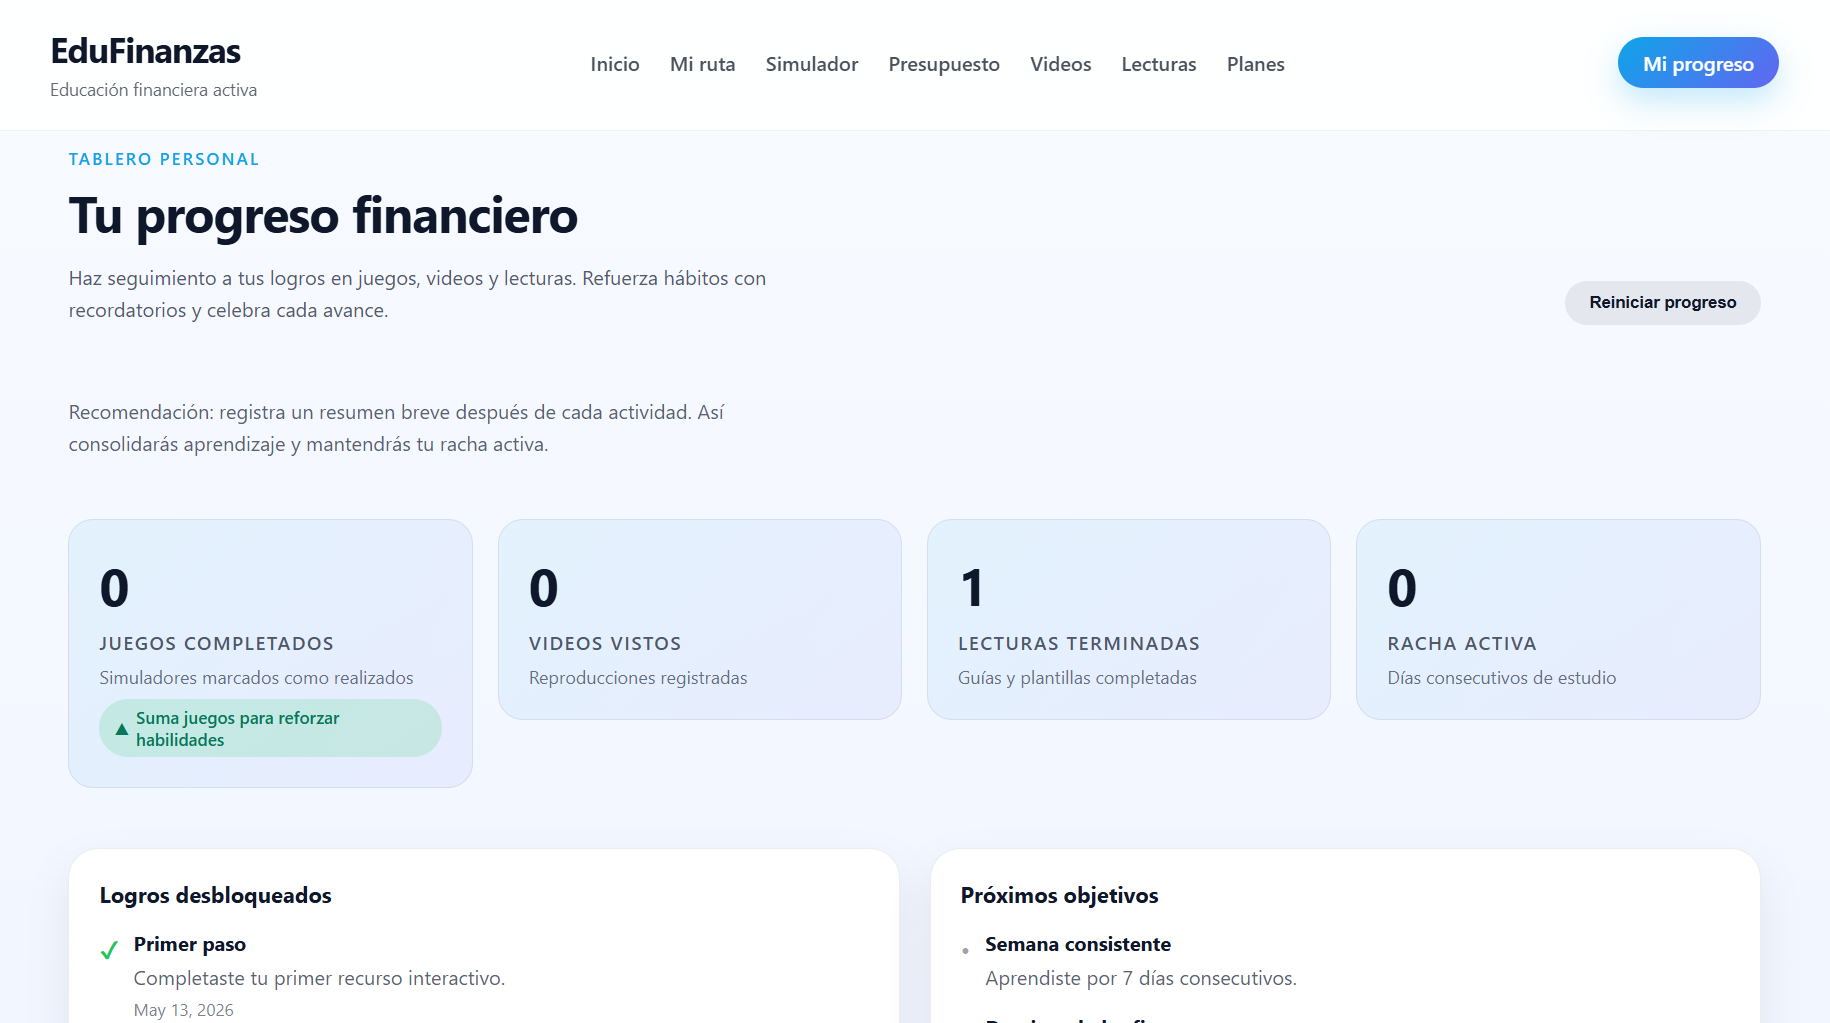
\includegraphics[width=15cm]{Imagenes/progreso.png}
	\caption[{Vista de la página de progreso.}]{\centering Vista de la página de progreso. \textit{Fuente:} Autores.}
	\label{fig:vistaprogreso}
\end{figure}

\begin{figure}[H]
	\centering
	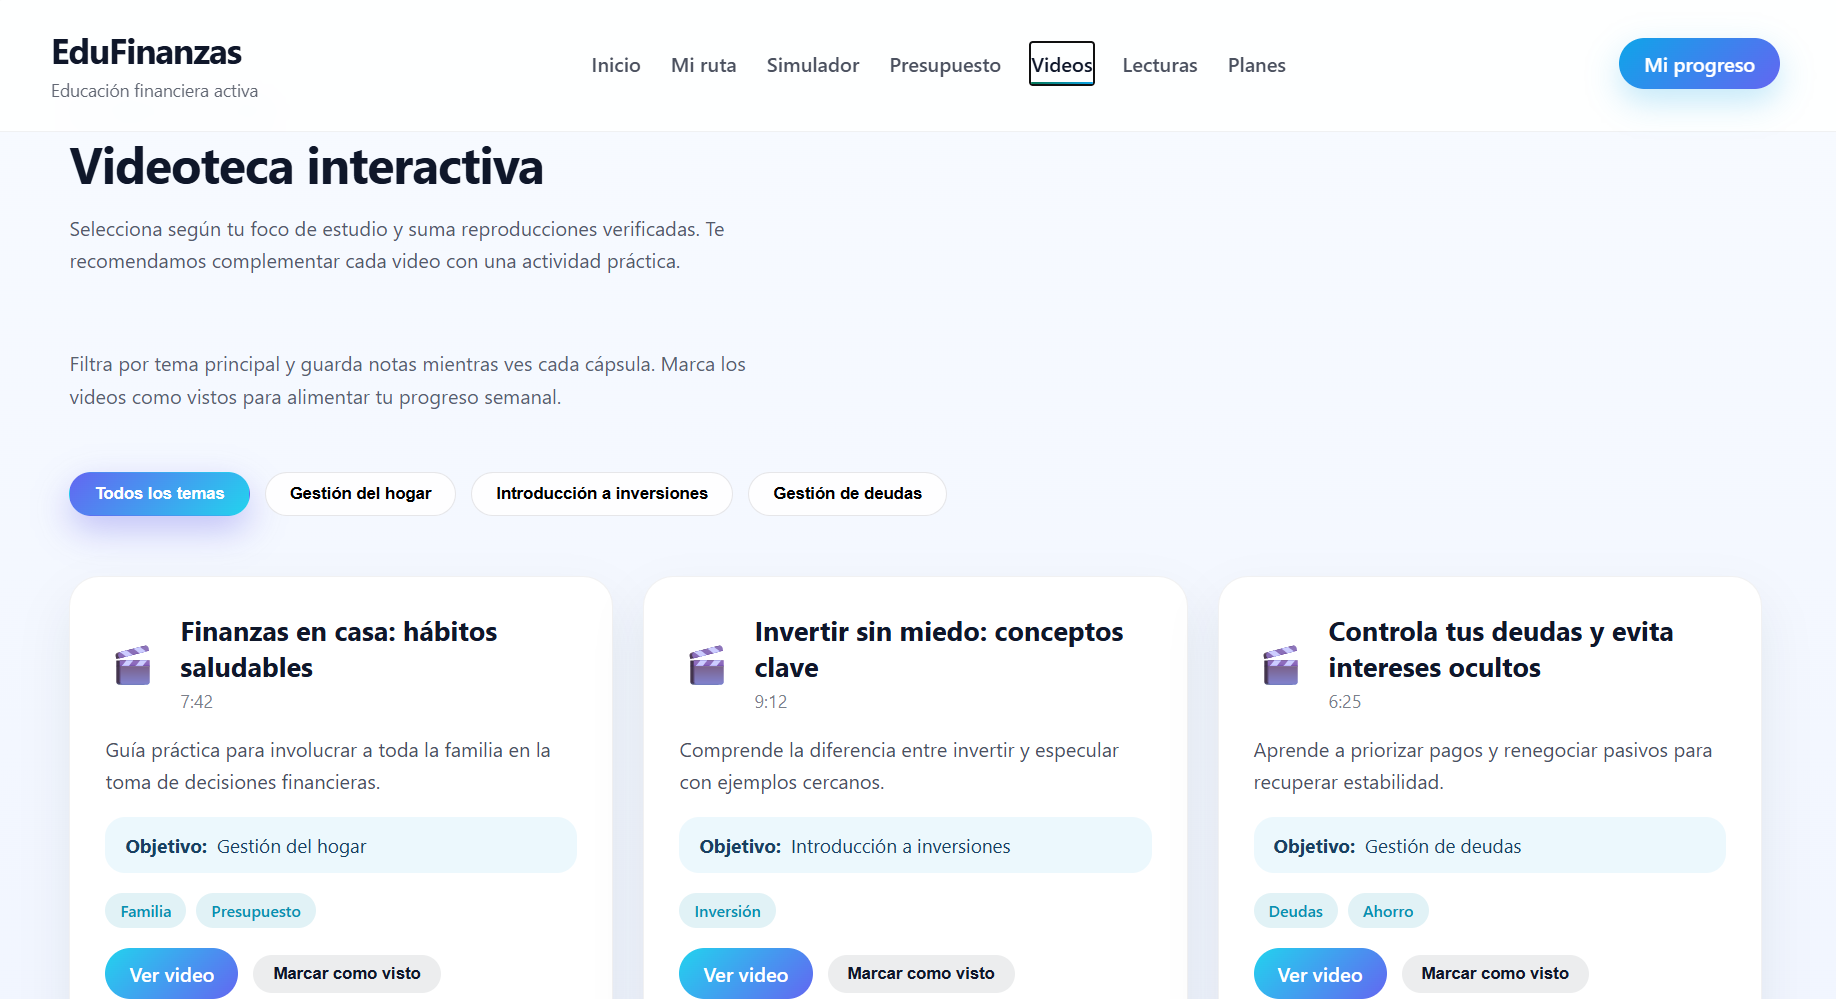
\includegraphics[width=15cm]{Imagenes/videoteca.png}
	\caption[{Vista de la página de videoteca.}]{\centering Vista de la página de videoteca. \textit{Fuente:} Autores.}
	\label{fig:vistavideoteca}
\end{figure}

\begin{figure}[H]
	\centering
	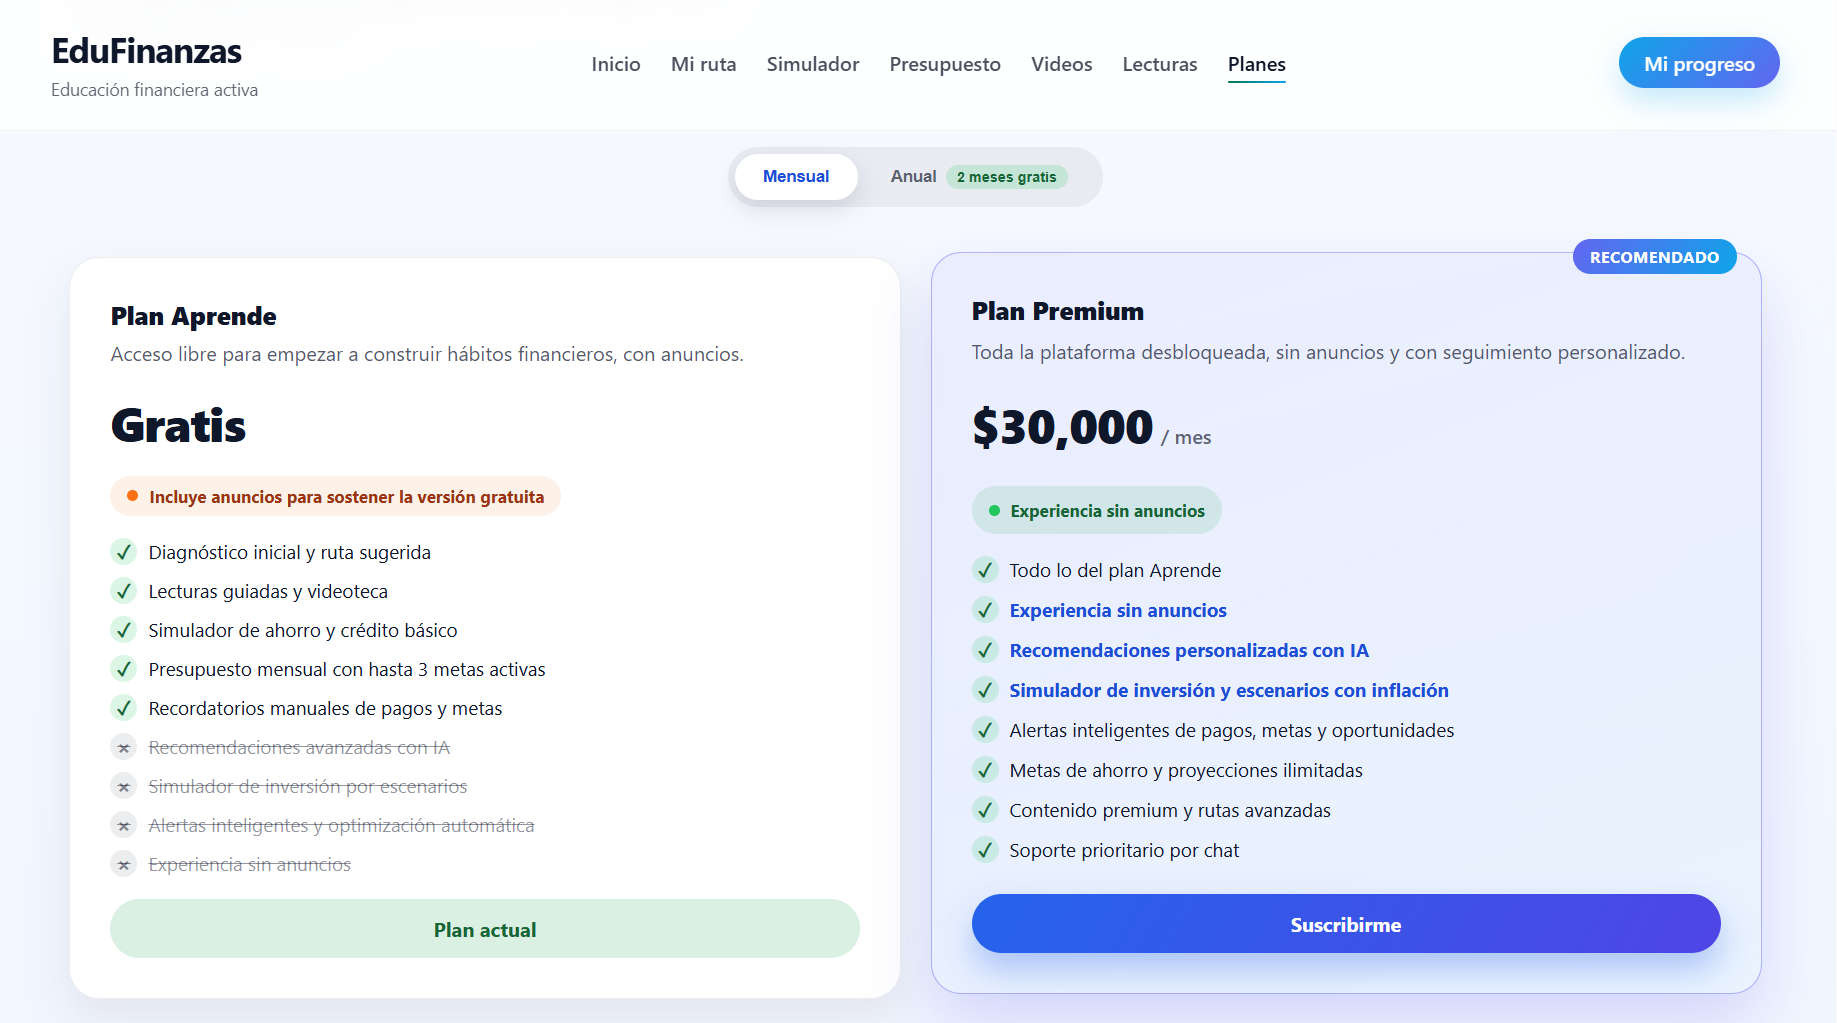
\includegraphics[width=15cm]{Imagenes/planes.png}
	\caption[{Vista de la página de planes.}]{\centering Vista de la página de planes. \textit{Fuente:} Autores.}
	\label{fig:vistaplanes}
\end{figure}

\begin{figure}[H]
	\centering
	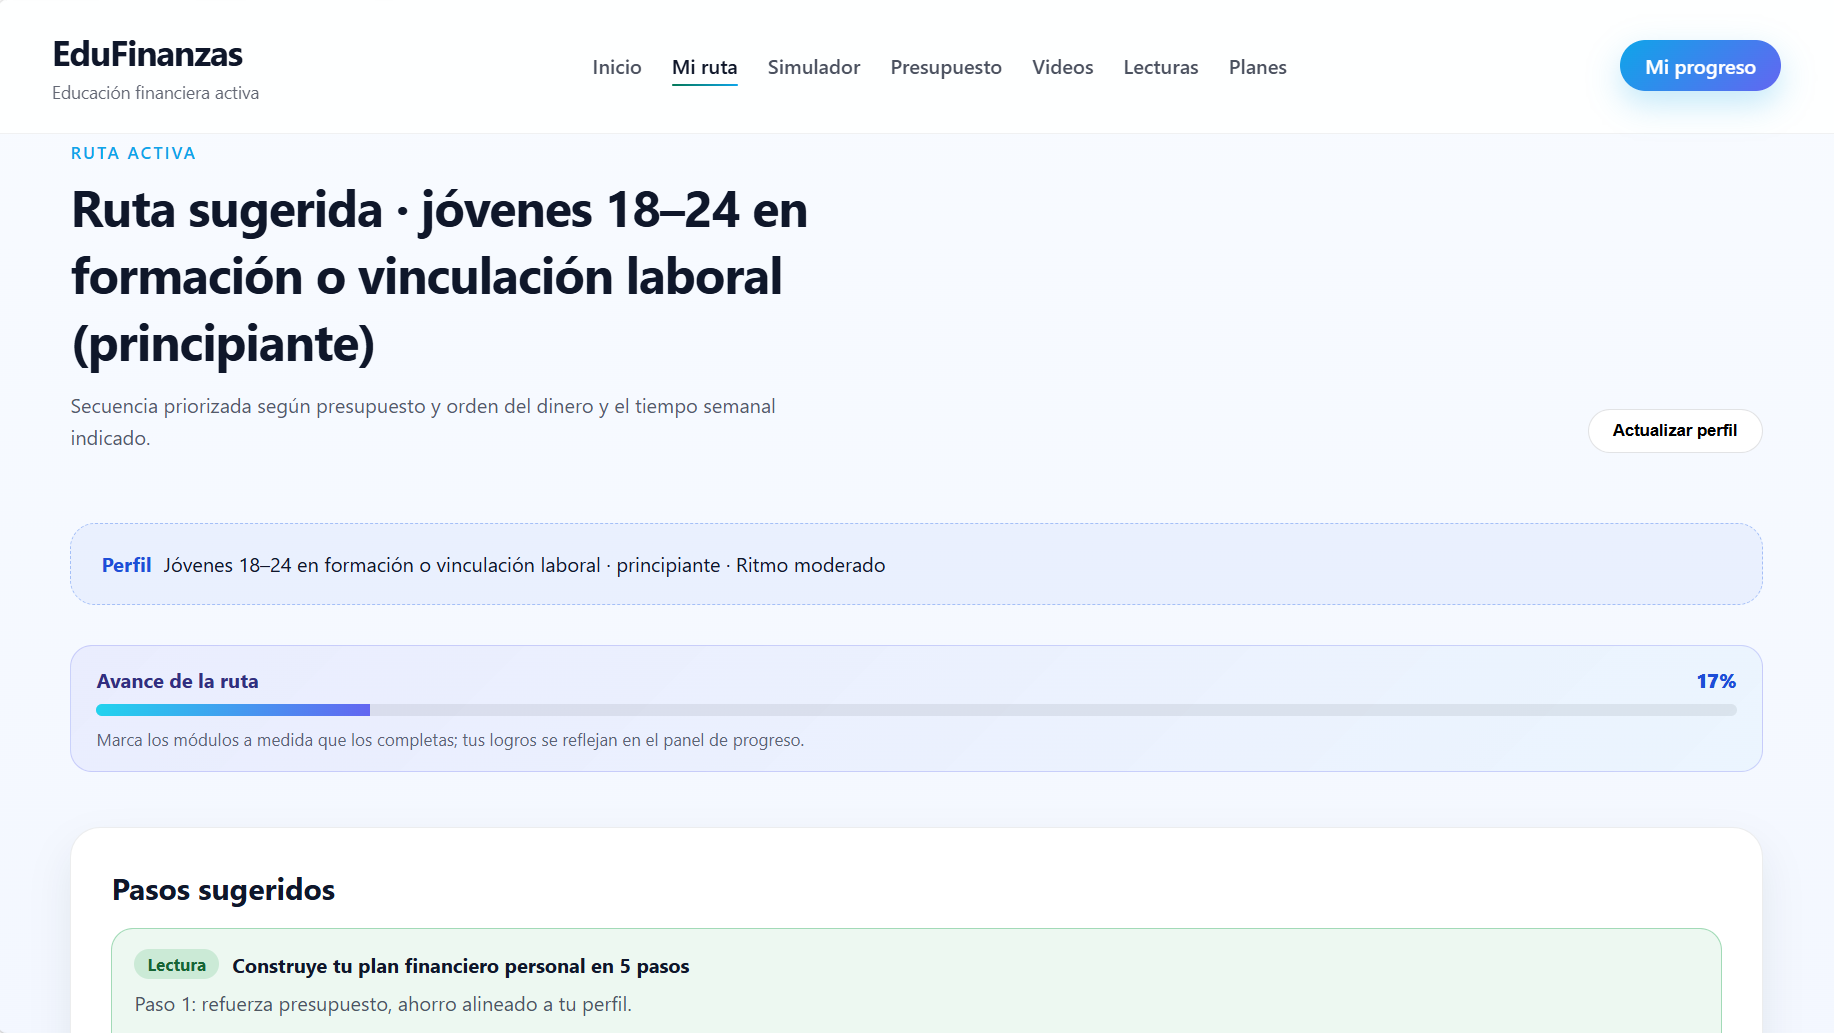
\includegraphics[width=15cm]{Imagenes/ruta.png}
	\caption[{Vista de la página de ruta de aprendizaje.}]{\centering Vista de la página de ruta de aprendizaje. \textit{Fuente:} Autores.}
	\label{fig:vistaruta}
\end{figure}